\documentclass{article}

% ------------------------------------ %
%             Document Info            %
% ------------------------------------ %

\usepackage{../../LaTeX-Preamables/Clean}
\newcommand{\documentdate}{Spring 2024}
\newcommand{\documenttype}{Notes}

% ------------------------------------ %
%              Title page              %
% ------------------------------------ %
\begin{document}
\begin{titlepage}
    \null\vfill % Add vertical space to center the title and author

    \centering
    \Huge\textbf{\documentname}

    \vspace{0.1cm}
    \Large\textbf{\documenttype\ $\cdot$ \documentdate}

    \vspace{1cm}
    \normalsize\textbf{Author:} \documentauthor

    \normalsize\textbf{Contact:} \documentauthorcontact

    MORE notes on my \href{https://jaxtam.dev/notes}{website}!
    \vfill % Add vertical space to center the remaining space
    \textcolor{gray}{Made for personal use only. Unmodified re-distribution is allowed. Content for reference only.}
\end{titlepage}

% ------------------------------------ %
%               Document               %
% ------------------------------------ %

\begin{center}
  Credit: Heavily inspired by \href{https://tutorial.math.lamar.edu/Classes/CalcI/CalcI.aspx}{Paul's Calculus I Notes}.
\end{center}

\section{Limits and Continuity}

\subsection{Introduction to the concept of limit}
\begin{minipage}{0.65\textwidth}
  We can conceptualize that the limit of a function $f(x)$ is $L$ as $x$ approaches $c$, given that we can make $f(x)$ \emph{as close to $L$ as we want} for all $x$ sufficiently close to $a$, from both sides, \emph{without actually letting $x$ be $a$}. We can write this as:
  \[\lim_{x\to a}f(x)=L\]
\end{minipage}
\hfill
\begin{minipage}{0.3\textwidth}
  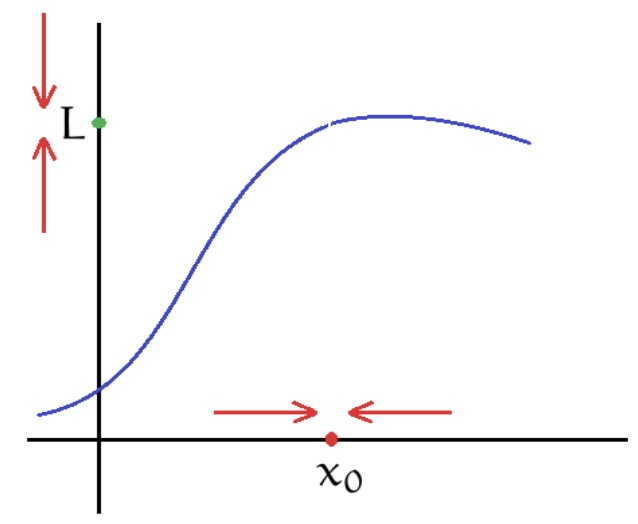
\includegraphics[width=\textwidth]{img/Lim.jpg}
\end{minipage}

\subsection{One-sided limits}
There are two sides that $x$ can tend to a number. We can write it as $x\to n^-$ and $x\to n^+$, which represents from the negative (left) / positive (right) side.

\subsection{Existence of limits}
\begin{theorem}
  {Condition for limit to exist}
  The limit for a function $f(x)$ only exists if and only if:
  \[\lim_{x\to a^+}f(x)=\lim_{x\to a^-}f(x)\]
\end{theorem}

\begin{minipage}{0.65\textwidth}
  For this example, when $x\to 0^-, y\to -\infty$.

  Similarly, as $x\to 0^+, y\to +\infty$.

  Hence, we can conclude that the limit for this function as $x\to 0$ doesn't exist.
\end{minipage}
\hfill
\begin{minipage}{0.25\textwidth}
  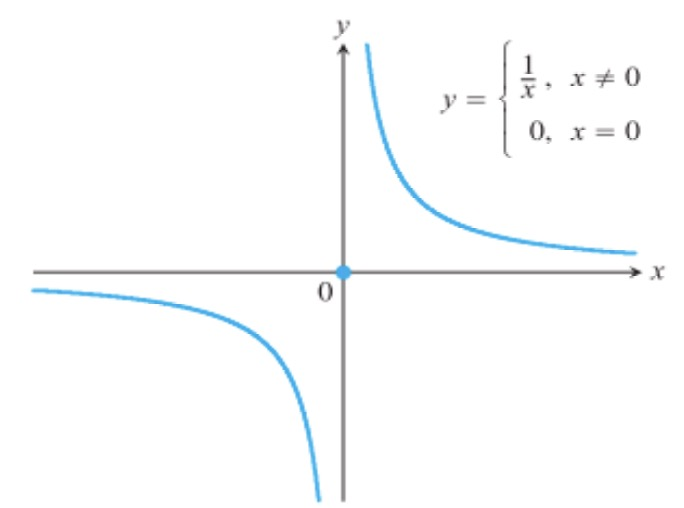
\includegraphics[width=\textwidth]{img/lim3.jpg}
\end{minipage}

\subsection{Continuity}
\begin{theorem}
  {Continuity}
  A function $f(x)$ is \emph{continuous} at $x=a$ if:
  \[\mathop {\lim }\limits_{x \to a} f\left( x \right) = f\left( a \right)\]
\end{theorem}
\begin{theorem}
  {Intermediate value theorem}
  If a function $f$ is continuous on $[a, b]$, there is a number $c$ in $[a, b]$ where $f(c)$ in $[f(a), f(b)]$.
\end{theorem}

\subsection{Computing limits}
\begin{theorem}
  {Using the limit laws}
  For functions $f,g$ and using $\mathop {\lim }\limits_{x \to a}=\bigcirc$ for simpler notation:
  \begin{enumerate}
    \item $lim_{x\to a}c=c$
    \item $\bigcirc(f\pm g)=\bigcirc f\pm \bigcirc g$
    \item $\bigcirc(k\cdot f)=k\cdot\bigcirc L$
    \item $\bigcirc(f^n)=(\bigcirc f)^n$
    \item $\bigcirc(fg)=\bigcirc f\bigcirc g$
    \item $\bigcirc(\frac{f}{g})=\frac{\bigcirc f}{\bigcirc g},\quad\text{given that }\bigcirc g\ne 0$. \emph{This strict condition prevents indeterminate forms.}
  \end{enumerate}
  We can use these laws to break a limit into separate limits, and compute that way. Also note that:
  \begin{enumerate}[start=7]
    \item $\bigcirc f(g)=f(\bigcirc g),\quad$given that $f$ is \textbf{continuous} at $\bigcirc g$
  \end{enumerate}
\end{theorem}
\begin{theorem}
  {Limit of a polynomial}
  For the limit of a polynomial $p(x)$:
  \[lim_{x\to a}p(x)=p(a)\]
  This can be proven easily with the limit laws above.
\end{theorem}
\begin{knBox}
  {Techniques to compute limits}
  To solve for limits, we have to get the expression to the right form - a polynomial, for us to substitute our limit value into the function.

  To do this, often we have to \textbf{factorize} or \textbf{rationalize}.
\end{knBox}
\begin{example}
  Indeterminate forms by substitution

  This applies limit law \#5. As substituting into the function directly gives $0/0$, we have to change it into a form such that we could apply the limit laws directly.
  \begin{align*}
    lim_{x\to 2}\frac{x^2+4x-12}{x^2-2x} & =\frac{(x-2)(x+6)}{(x-2)x} \\
                                         & =\frac{x+6}{x}             \\
    \text{Substituting 2 gives}          & =4
  \end{align*}
\end{example}


\begin{theorem}
  {The squeeze / sandwich theorem}
  Suppose $f(x)\le g(x) \le h(x)$ in the range $[a, b]$, for $c$ in $[a, b]$:
  \[\lim_{x\to c}f \le \lim_{x\to c}g \le \lim_{x\to c}h\]
  We will make use of the fact that the limits can be equal to solve for the limit of $g(x)$.
\end{theorem}

\begin{example}
  Squeezing a function

  When we can't seem to factorize a function, we can try squeezing it between two other functions.
  \[\lim_{x\to 0}x^2\cos\frac{1}{x}\]
  We know the limits of the function $\cos \frac{1}{x}$, so we can start from there.
  \[\text{Given that }x\ne 0, -1\le \cos \frac{1}{x} \le 1\]
  \[\text{Multiplying }x^2\text{ on both sides},-x^2\le \cos x^2\frac{1}{x} \le x^2\]
  \[\text{As }\lim_{x\to 0}\pm x^2=0,\quad\text{we can conclude that }\lim_{x\to 0}x^2\cos\frac{1}{x}=0\]
\end{example}

\subsection{Infinite limits}
\begin{knBox}
  {Determining infinite limits}
  If $f(x)$ gets (negatively) arbitrarily large when $x$ approaches $a$, we can say:
  \[\lim_{x\to a}f(x)=(-)\infty\]
  After we know that the limit \emph{may} be infinity, we then have to make sure that \emph{the limit is the same from both sides}, so that the limit actually exists. We can do so by plugging numbers which are approaching the limit from both sides.
\end{knBox}

\begin{minipage}{0.45\textwidth}
  \begin{example}
    Infinite limit exists
    \[\lim_{x\to 0}\frac{6}{x^2}\]
    \[\text{Consider both}\ \lim_{x\to 0^-}\frac{6}{x^2},\lim_{x\to 0^+}\frac{6}{x^2}:\]
    \[\lim_{x\to 0}\frac{6}{x^2}=\infty\]
  \end{example}
\end{minipage}
\hfill
\begin{minipage}{0.45\textwidth}
  \vspace{10pt}
  \begin{example}
    Infinite limit doesn't exist
    \[\lim_{x\to 4}\frac{3}{(4-x)^3}\]
    \begin{center}
      Checking both sides, we can conclude that the limit doesn't exist, as:
    \end{center}
    \[\lim_{x\to 4^+}\frac{3}{(4-x)^3}=-\infty,\quad\lim_{x\to 4^-}\frac{3}{(4-x)^3}=\infty\]
  \end{example}
\end{minipage}

\subsection{Limits at infinity}
\begin{theorem}
  {Infinity operations}
  Note the following operations:
  \begin{enumerate}
    \item $\infty + k=\infty$
    \item For $k<0,\ k\infty=-\infty$
  \end{enumerate}
\end{theorem}
\begin{knBox}
  {Determining limits of infinity}
  It is not hard to see that, for rational numbers $n$:
  \[\lim_{x\to\pm\infty}\frac{k}{x^n}=0\]
  The easiest way to determine the limit would be to \emph{factorize} the function so that we can use the facts above.
\end{knBox}
\begin{theorem}
  {Determining limits of infinity of polynomials}
  Using the above fact, we can produce the fact, for a polynomial $p(x)$ with degree $n$ and largest coefficient $a_n$:
  \[\lim_{x\to\pm\infty}p(x)=a_nx^n\]
  Which means we can \emph{only consider the largest term in a polynomial} for limits of infinity.
\end{theorem}
\begin{example}
  Indeterminate forms by substitution of infinity

  Substituting $\infty$ into the function gives $\infty-\infty-\infty$, which is indeterminate. Hence, we must factorize it.
  \begin{align*}
    \lim_{x\to\infty}2x^4-x^2-8x & =\lim_{x\to\infty}[x^4(2-\frac{1}{x^2}-\frac{8}{x^3})] \\
                                 & =\infty\times 2                                        \\
                                 & =\infty
  \end{align*}
  Or we can just simply use the theorem above and consider $\lim_{x\to\infty}2x^4$ only to give $\infty$.
\end{example}
\begin{example}
  Factor polynomials limit to infinity

  We can simply consider the largest terms on each side and give the final answer easily.
  \begin{align*}
    \lim_{x \to -\infty } \frac{{\sqrt {3{x^2} + 6} }}{{5 - 2x}} & =\lim_{x \to \infty }\frac{\sqrt{3x^2}}{-2x} \\
                                                                 & =\lim_{x \to \infty }\frac{\sqrt{3}|x|}{-2x} \\
                                                                 & =\frac{-\infty\sqrt{3}}{-2\times\infty}      \\
                                                                 & =\frac{\sqrt{3}}{2}
  \end{align*}
  Note that, as we are considering the negative limit of infinity, we need to add - to the abs sign on line 3.
\end{example}

% \subsection{The theorem of limit}
% \begin{theorem}
%   {Limit}
%   \[\text{if there are numbers such that }\left| {f\left( x \right) - L} \right| < \varepsilon \quad{\mbox{whenever}}\quad0 < \left| {x - a} \right| < \delta\]
%   \[\mathop {\lim }\limits_{x \to a} f\left( x \right) = L\]
% \end{theorem} 

\section{Derivatives}
\begin{theorem}[]{First principle}
  \begin{flalign*}
    f'(x) & = \frac{d}{dx} f(x)=\lim_{h\to 0}\frac{f(x+h)-f(x)}{h} &
  \end{flalign*}
\end{theorem}

\subsection{Differentiation formulas and rules}
\begin{knBox}
  {Basic formulas}
  \begin{itemize}
    \item We can differentiate individual items: $\displaystyle {\left( {f \pm g} \right)^\prime } = f' \pm g'$
    \item We can factor out a multiplicative constant: $\displaystyle {\left( {cf} \right)^\prime } = cf'$
    \item Derivative of a constant is 0: $\frac{d}{dx}k = 0$
    \item Power rule: $\frac{d}{dx}x^n = nx^{n-1}$
  \end{itemize}

\end{knBox}
\begin{minipage}{0.65\textwidth}
  \begin{theorem}
    {Chain rule}
    Shorthand: \textbf{d}1x2 + \textbf{d}2x1
    \[(u(v))'=u'(v)v'\quad\quad\text{or}\quad\quad\frac{dy}{dx}=\frac{dy}{du}\frac{du}{dx}\]
  \end{theorem}
  \begin{theorem}
    {Product rule}
    Shorthand: \textbf{d} from outside to inside
    \[(uv)' = uv' + vu'\quad\quad\text{or}\quad\quad\frac{d}{dx}(uv)=u\frac{dv}{dx}+v\frac{du}{dx}\]
  \end{theorem}
  \begin{theorem}
    {Quotient rule}
    Shorthand: move lower \textbf{d} upper - \textbf{d} lower x upper, lower square
    \[(\frac{u}{v})'=\frac{vu'-uv'}{v^2}\quad\quad\text{or}\quad\quad\frac{d}{dx}(\frac{u}{v})=\frac{v\frac{du}{dx}-u\frac{dv}{dx}}{v^2}\]
  \end{theorem}
\end{minipage}
\hfill
\begin{minipage}{0.25\textwidth}
  \begin{table}[H]
    \begin{tabular}{rcc}
          & $f(x)$    & $f'(x)$           \\ \hline
      1.  & $a^x$     & $\ln{a}\cdot a^x$ \\ \arrayrulecolor{lightgray}\hline
      2.  & $e^{kx}$  & $ke^{kx}$         \\ \arrayrulecolor{lightgray}\hline
      3.  & $\ln{kx}$ & $x^{-1}$          \\ \arrayrulecolor{lightgray}\hline
      4.  & $\sin kx$ & $k\cos kx$        \\ \arrayrulecolor{lightgray}\hline
      5.  & $\cos kx$ & $-k\sin kx$       \\ \arrayrulecolor{lightgray}\hline
      6.  & $|x|$     & $\frac{|x|}{x}$   \\ \arrayrulecolor{lightgray}\hline
      7.  & $\tan kx$ & $k\sec^2 kx$      \\ \arrayrulecolor{lightgray}\hline
      8.  & $\csc x$  & $-\csc x \cot x$  \\ \arrayrulecolor{lightgray}\hline
      9.  & $\sec x$  & $\sec x \tan x$   \\ \arrayrulecolor{lightgray}\hline
      10. & $\cot x$  & $-\csc^2x$
    \end{tabular}
  \end{table}
\end{minipage}
\begin{knBox}
  {Implicit differentiation}
  Differentiate all $xy$, add $\frac{dy}{dx}$ behind all differentiations of $y$.
  \tcblower
\end{knBox}






\subsection{Implicit differentiation}
\subsection{Differentiation formulas for natural logarithms \& exponential functions}
\subsection{Logarithmic Differentiation}
\subsection{Extremum points}
\subsection{The Mean Value Theorem \& its consequences}
\subsection{Monotonicity and the First Derivative}
\subsection{Concavity and the Second Derivative}
\section{Integrals}
\subsection{Area and Estimating with Finite Sums}
\subsection{Definite Integrals}
\subsection{The Fundamental Theorem of Calculus}
\subsection{theorem of Natural Logarithms}
\subsection{Interlude - Hyperbolic Functions}
\section{Parametric Equations}
\section{Polar Coordinates}
\section{Ordinary Differential Equations}
\subsection{1st Order Linear ODEs \& Integrating Factors}
\subsection{Bernoulli Equations \& Riccati Equations}

\end{document}